\section{To-Be}
\label{sec:to_be}
This section will focus on the To-Be architecture of J.D.H. Insurance. Changes from the As-Is architecture and models and analysis of the target architecture to align the architecture with the strategy of the company and to approach the vision stated in this report will be presented. These changes are based on the improvement areas described in the previous section. The full To-Be architecture divided in business layer, application layer, infrastructure layer and information layer can be seen in Appendix B. Furthermore, the full architecture can be seen in the attached iEaat file JDHInsuranceToBe.
\subsection{Changes to core processes}
The changes to the core processes are described during this section.
\subsubsection{Order Process}
To lower the cost of the order registration process it has been transformed to an automated service on the website which eliminates the costs of the order manager and the order management systems. As the website is already available for browsing insurances, the cost for implementing the ordering service on the website is significantly smaller to the cost of todays employees and order management systems. Since the system for customer relation management has support for storing information about customer's insurances and customer information, this system replaces the order management system. Fewer systems and the usage of the website does not impact the service availability negatively and it makes it possible for the customers to use the service even at closed-office hours of the day. The websites functionality of browsing insurances remain and the change is made to the architecture supporting the Apply Order service. The customer is now able to send an order from the website and instead of receiving an order acceptance letter, the website directly presents the order acceptance. \Fref{fig:map_order_tobe} shows the new underlying architecture of the Apply order service and the full architecture of the Order process can be seen in the mentioned iEaat file in the view Order.
\begin{center}
	\begin{figure}[H]
		\centering
		\setlength\fboxsep{7pt}
		\setlength\fboxrule{0.5pt}
		\fbox{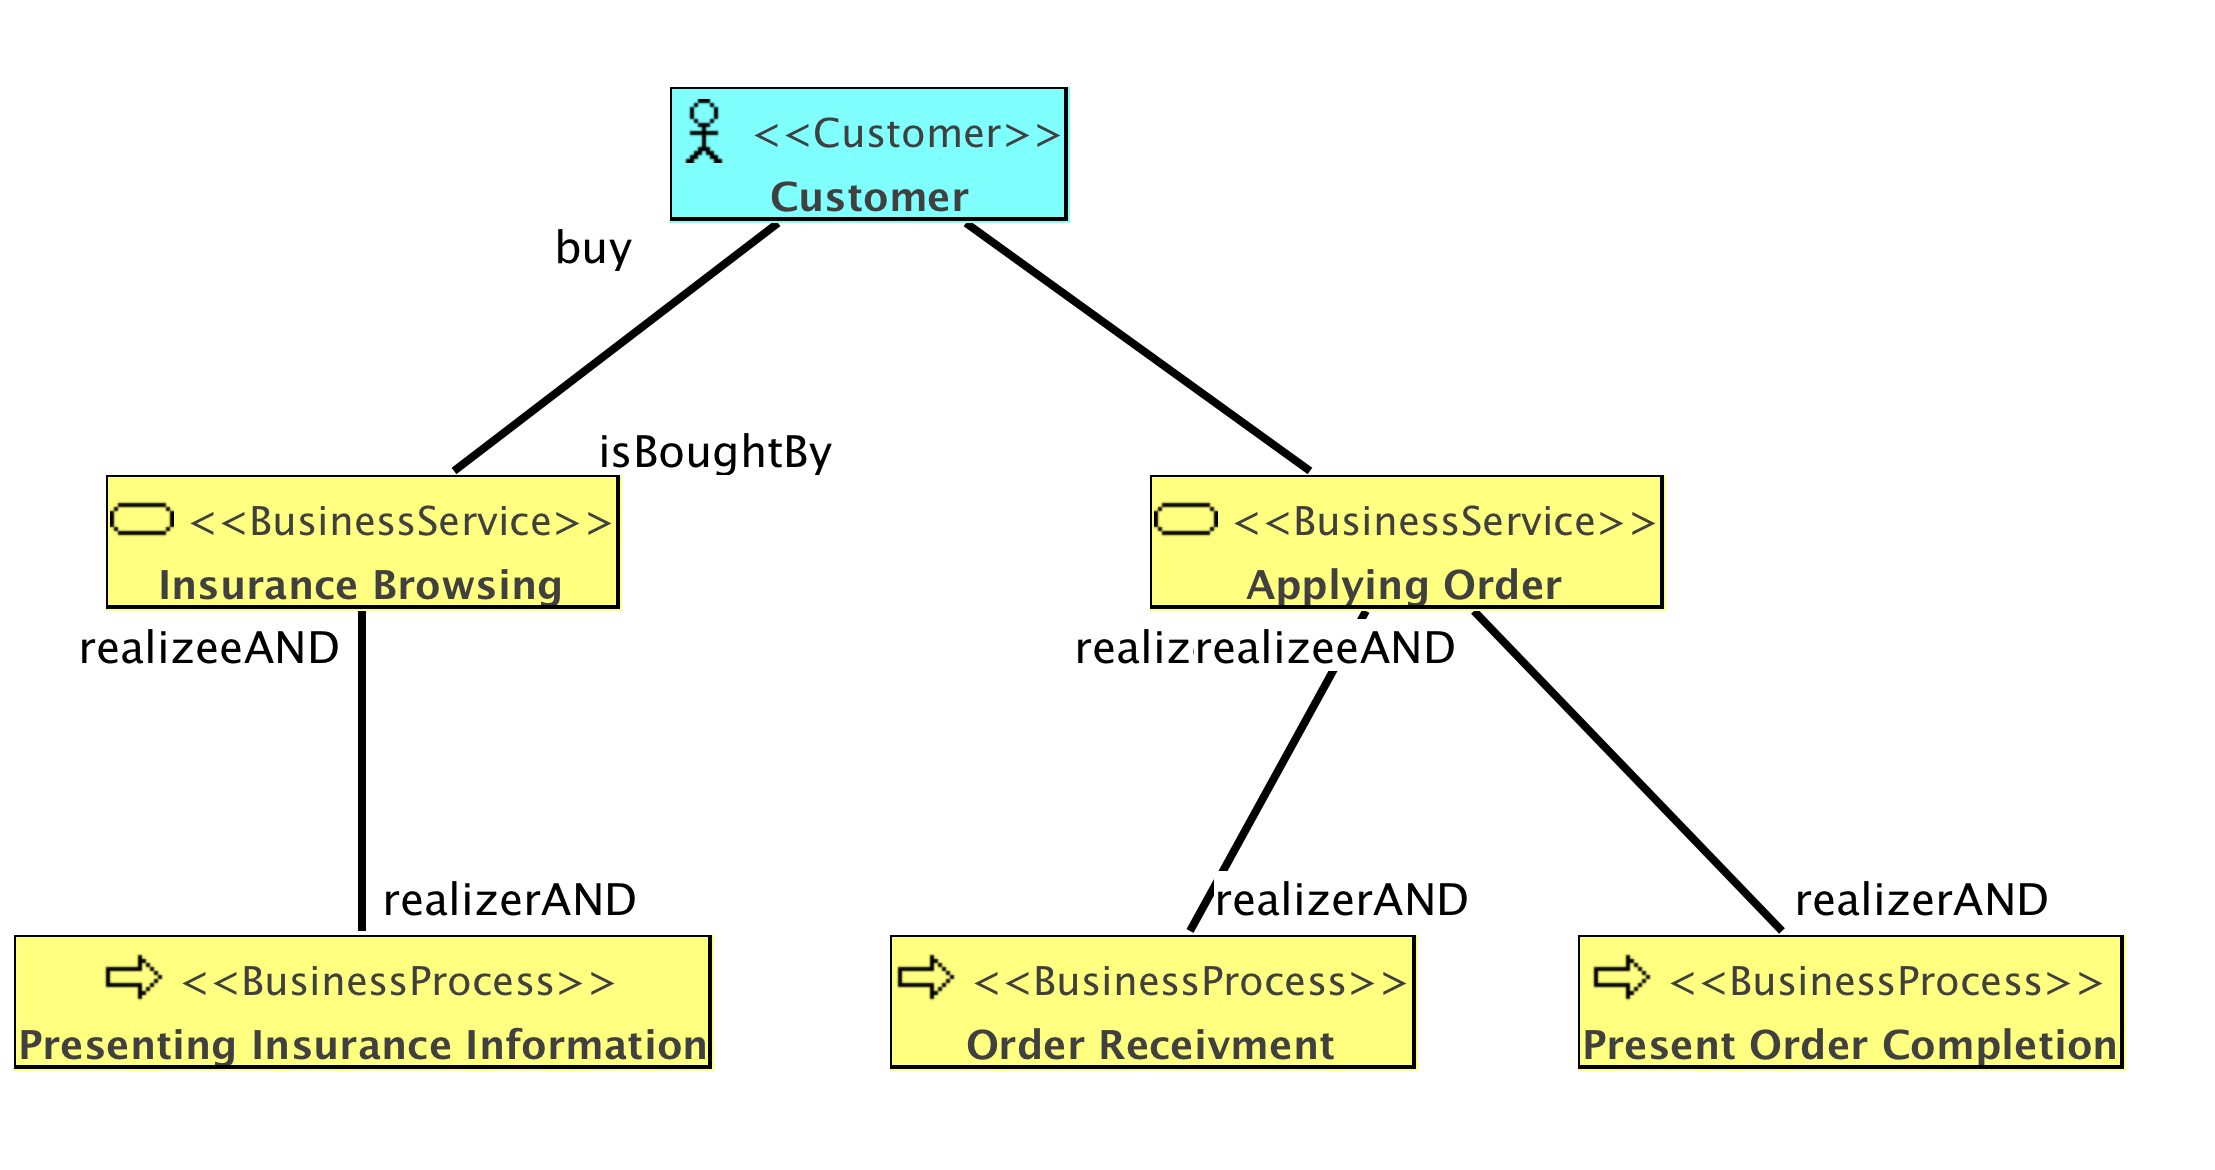
\includegraphics[scale = 0.15]{images/map_order_business_tobe.png}}
		\caption{Ordering an insurance}
		\label{fig:map_order_tobe}
	\end{figure}
\end{center}

\subsubsection{Claim Process}
To improve the accuracy of the claim registration process today's claim applications found on the website to print and send to the company is replaced by a web service. The big failure of the accuracy is the claim administrator who transforms these paper applications to a digital format using the claim management system, due to applications written by hand or interpretations. A web service registering the claim directly into the claim management database decreases the deterioration in the claim registration process. The function of the Claim evaluator will remain and the processes executed by her will not be affected by the change. The change is made in the architecture supporting the Claim Compensation Service. \Fref{fig:map_claim_tobe} displays the new architecture of that service and the full architecture of the Claim process can be seen in the mentioned iEaat file in the view Claim.
\begin{center}
	\begin{figure}[H]
		\centering
		\setlength\fboxsep{7pt}
		\setlength\fboxrule{0.5pt}
		\fbox{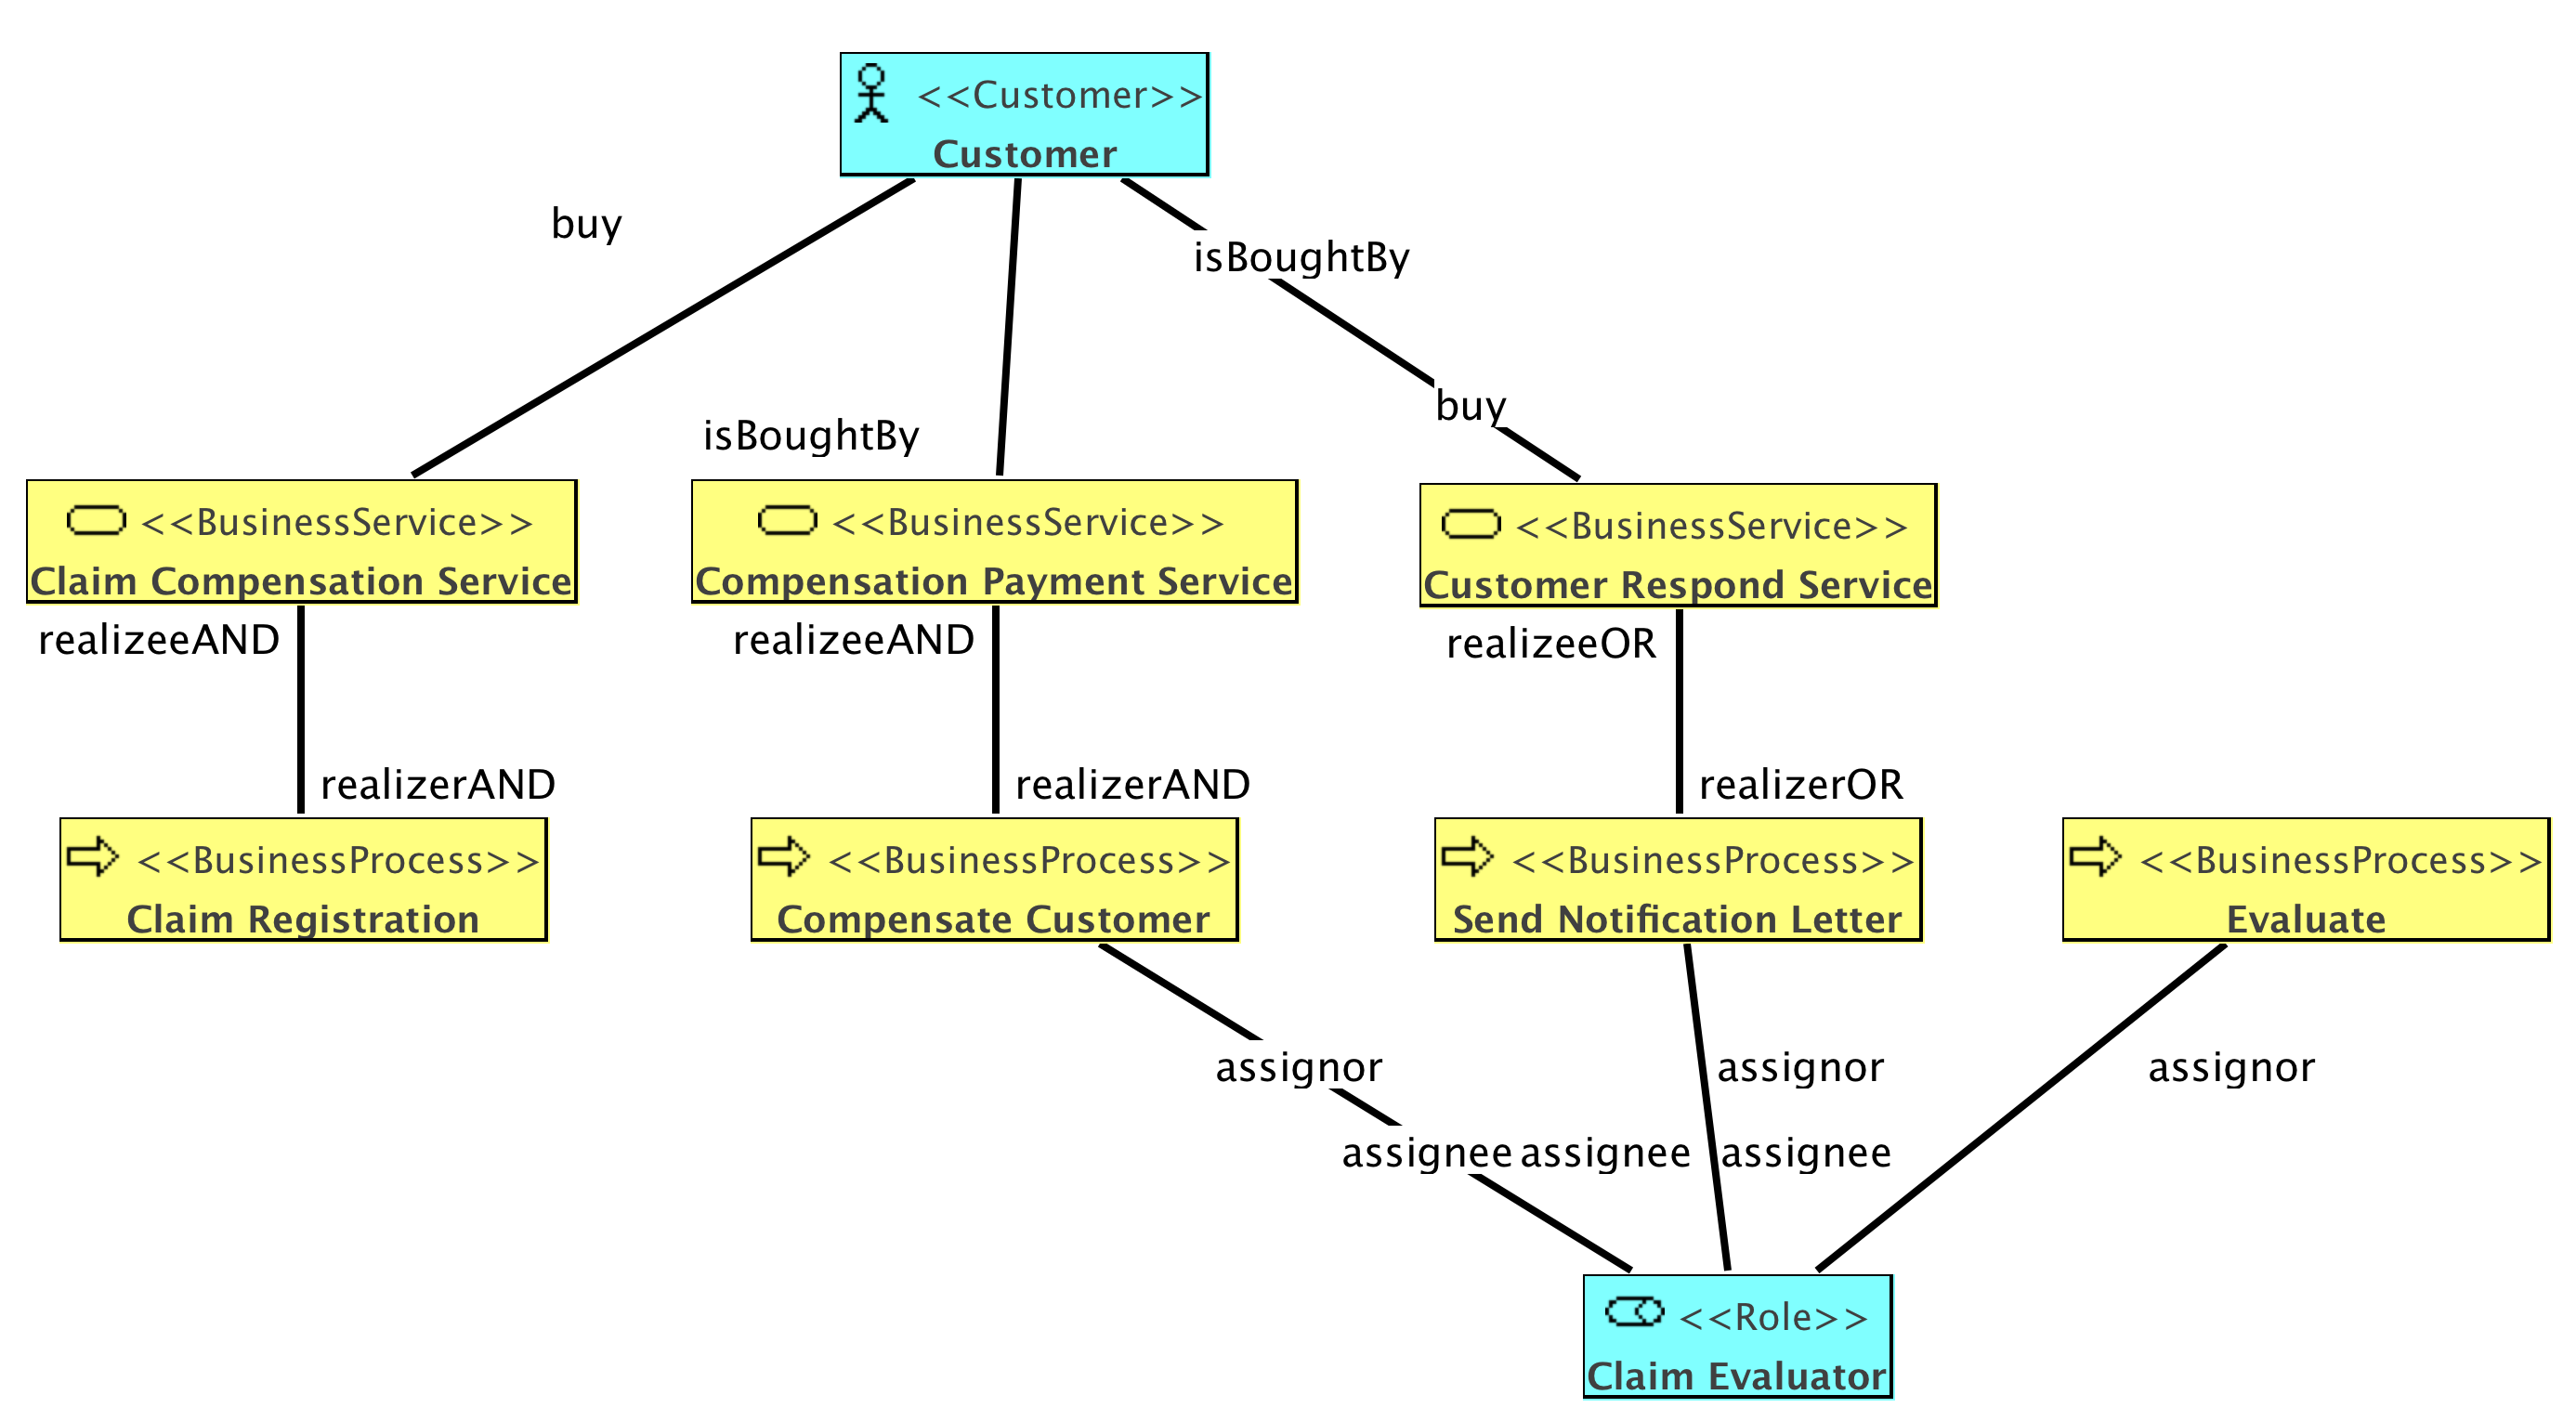
\includegraphics[scale = 0.15]{images/map_claim_business_tobe.png}}
		\caption{Claim registration}
		\label{fig:map_claim_tobe}
	\end{figure}
\end{center}
\subsubsection{Support Services}
As the availability of the mail support service and phone support system depend on different systems and on different employees, a aggregation of the two services increases the availability. As the phone support system is an old system and not as reliable as new systems, the new common Help desk system, handling both the phone support and the mail support will be easier to maintain and the availability will thereby increase. The phone dispatcher system and the mail server are still of use and will be integrated to this system. The Help desk system will be introduced to the current employees of both the mail and the phone support which will ensure higher flexibility of the employees, making it easier to replace them in case of absent employees. In \fref{fig:map_support_tobe}, the business layer of the new architecture is presented and in the mentioned iEaat file, the whole architecture for the Support service can be view in the Support view.
\begin{center}
	\begin{figure}[H]
		\centering
		\setlength\fboxsep{7pt}
		\setlength\fboxrule{0.5pt}
		\fbox{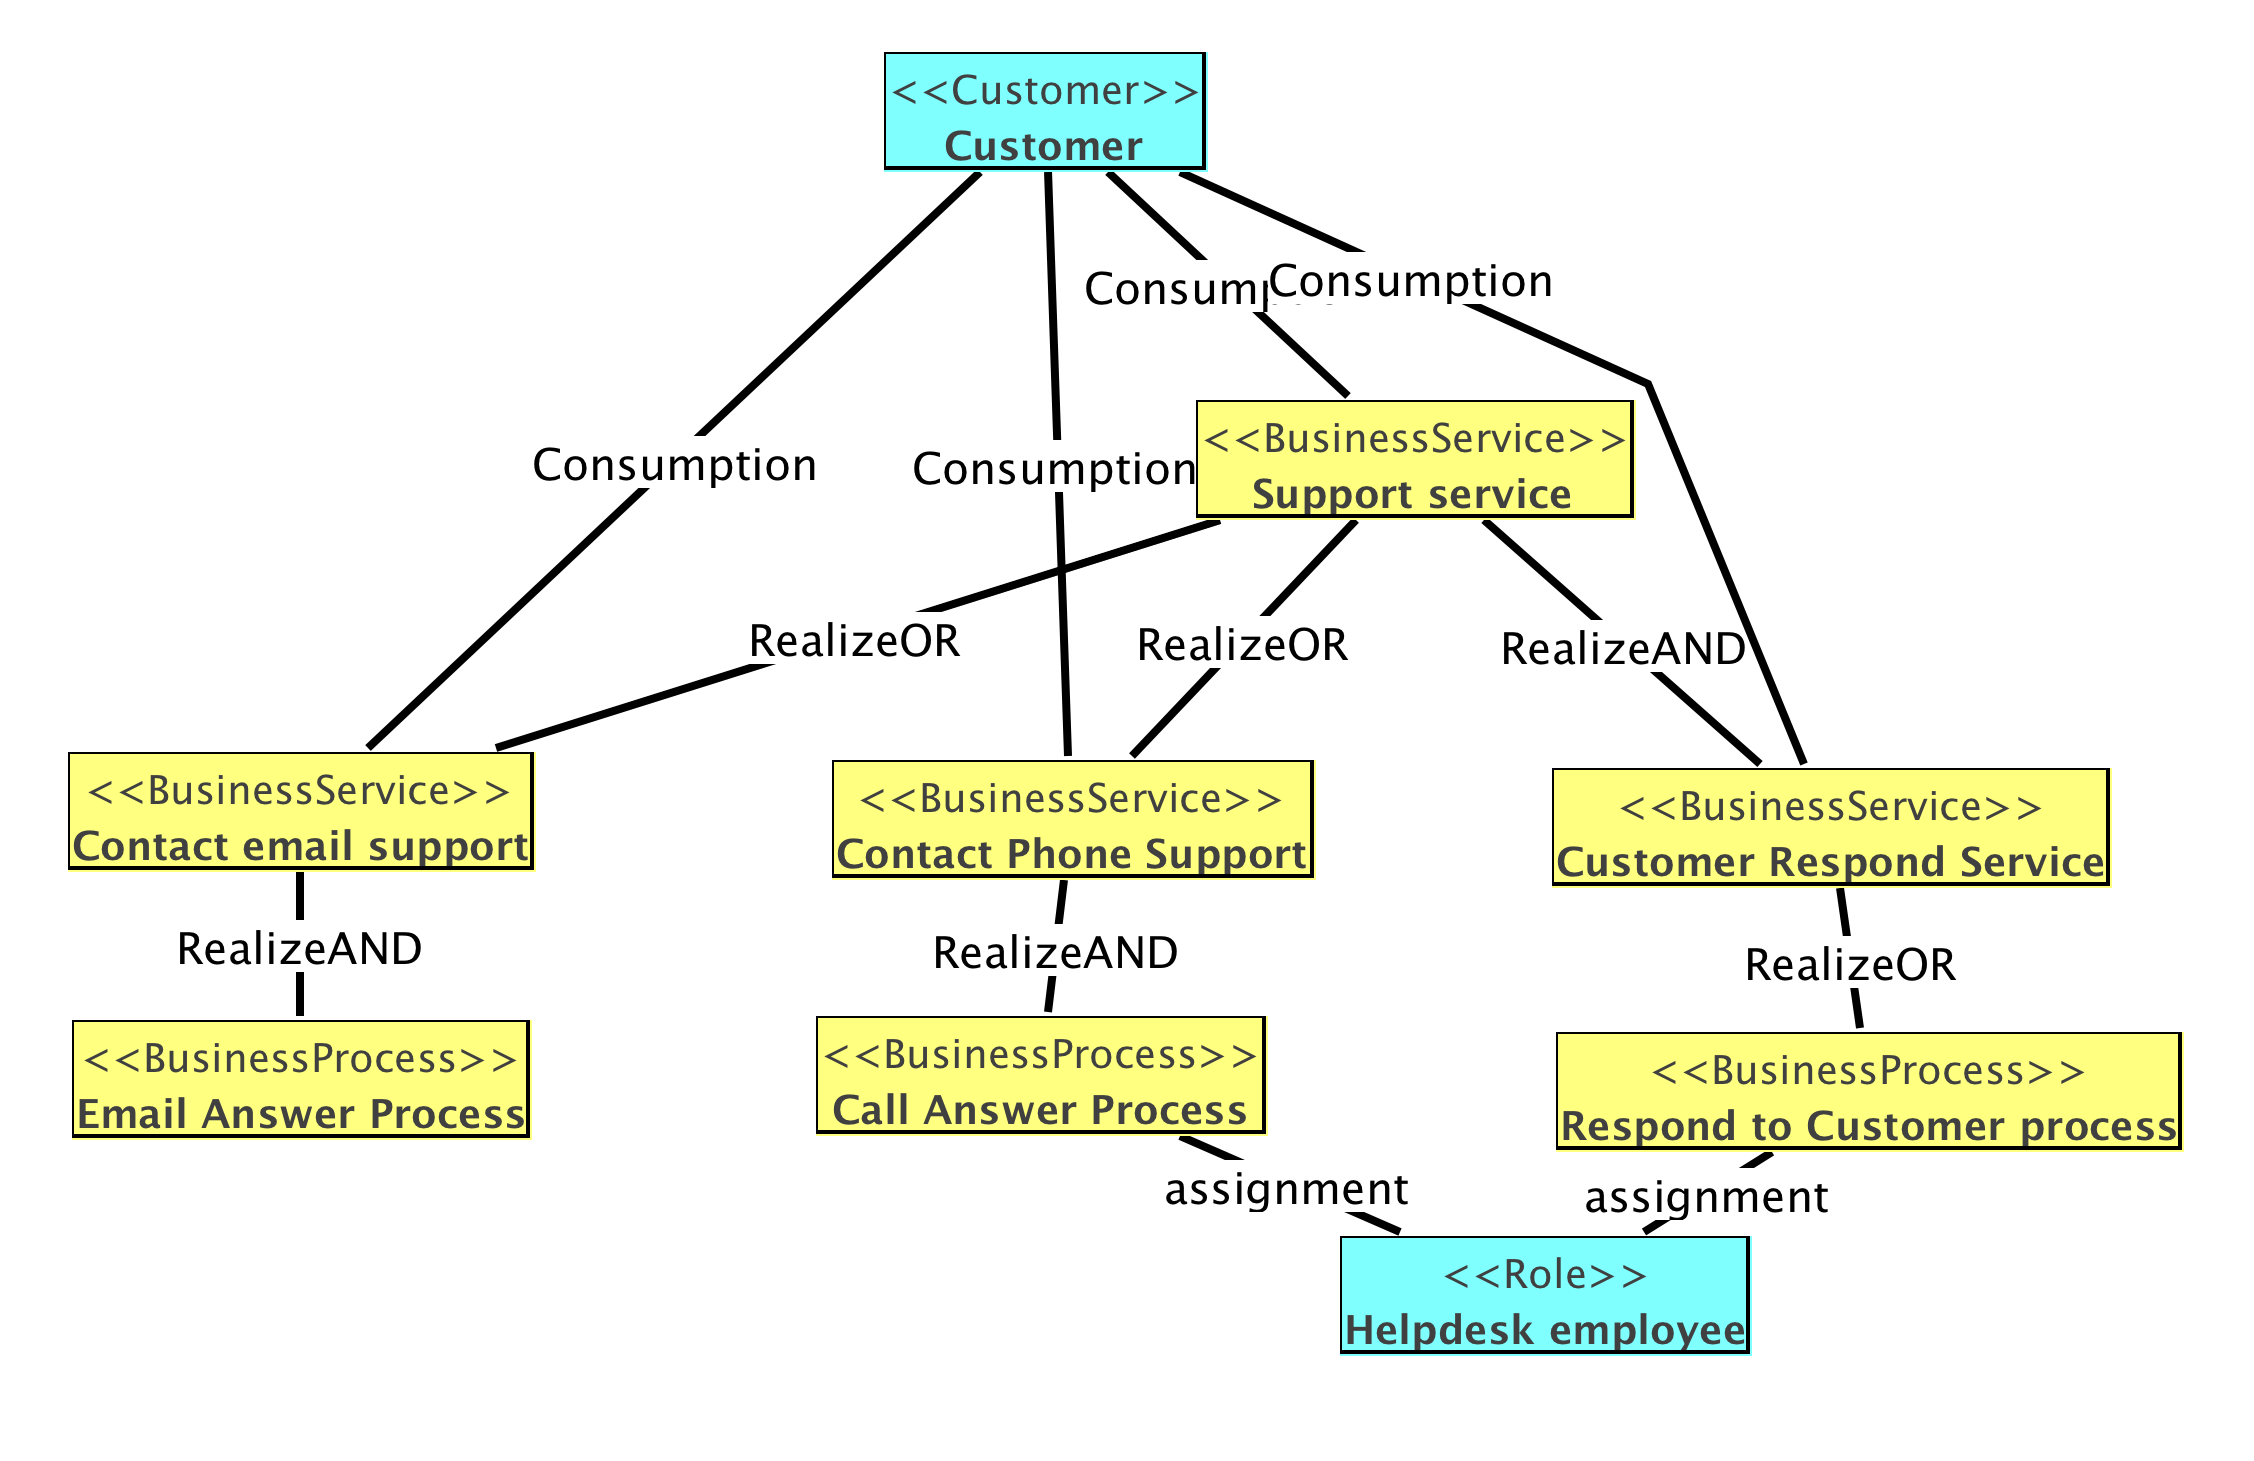
\includegraphics[scale = 0.15]{images/map_support_business_tobe.png}}
		\caption{Support process}
		\label{fig:map_support_tobe}
	\end{figure}
\end{center}
\subsection{MAP Analysis}
\label{sec:map_analysis_to_be}
Analysis of the new architectural changes to the enterprise will be presented in this section.
%
\subsubsection{Order Registration - Cost and Service Availability}
The changes from today's order registration process to the new processes supported by the web site impacts the cost of the whole registration process. The corresponding processes in the new architecture, Order Recievement and Present Order Completion to be seen in \fref{fig:map_order_cost_to_be}, are fully automated by the web site. \Fref{fig:map_order_cost_to_be} displays the objects of the order registration process analyzed. The analysis is made on both cost and availability, to ensure that the reduction of cost do not affect the availability of the process.
\label{sec:order_analysis}
\begin{center}
	\begin{figure}[H]
		\centering
		\setlength\fboxsep{7pt}
		\setlength\fboxrule{0.5pt}
		\fbox{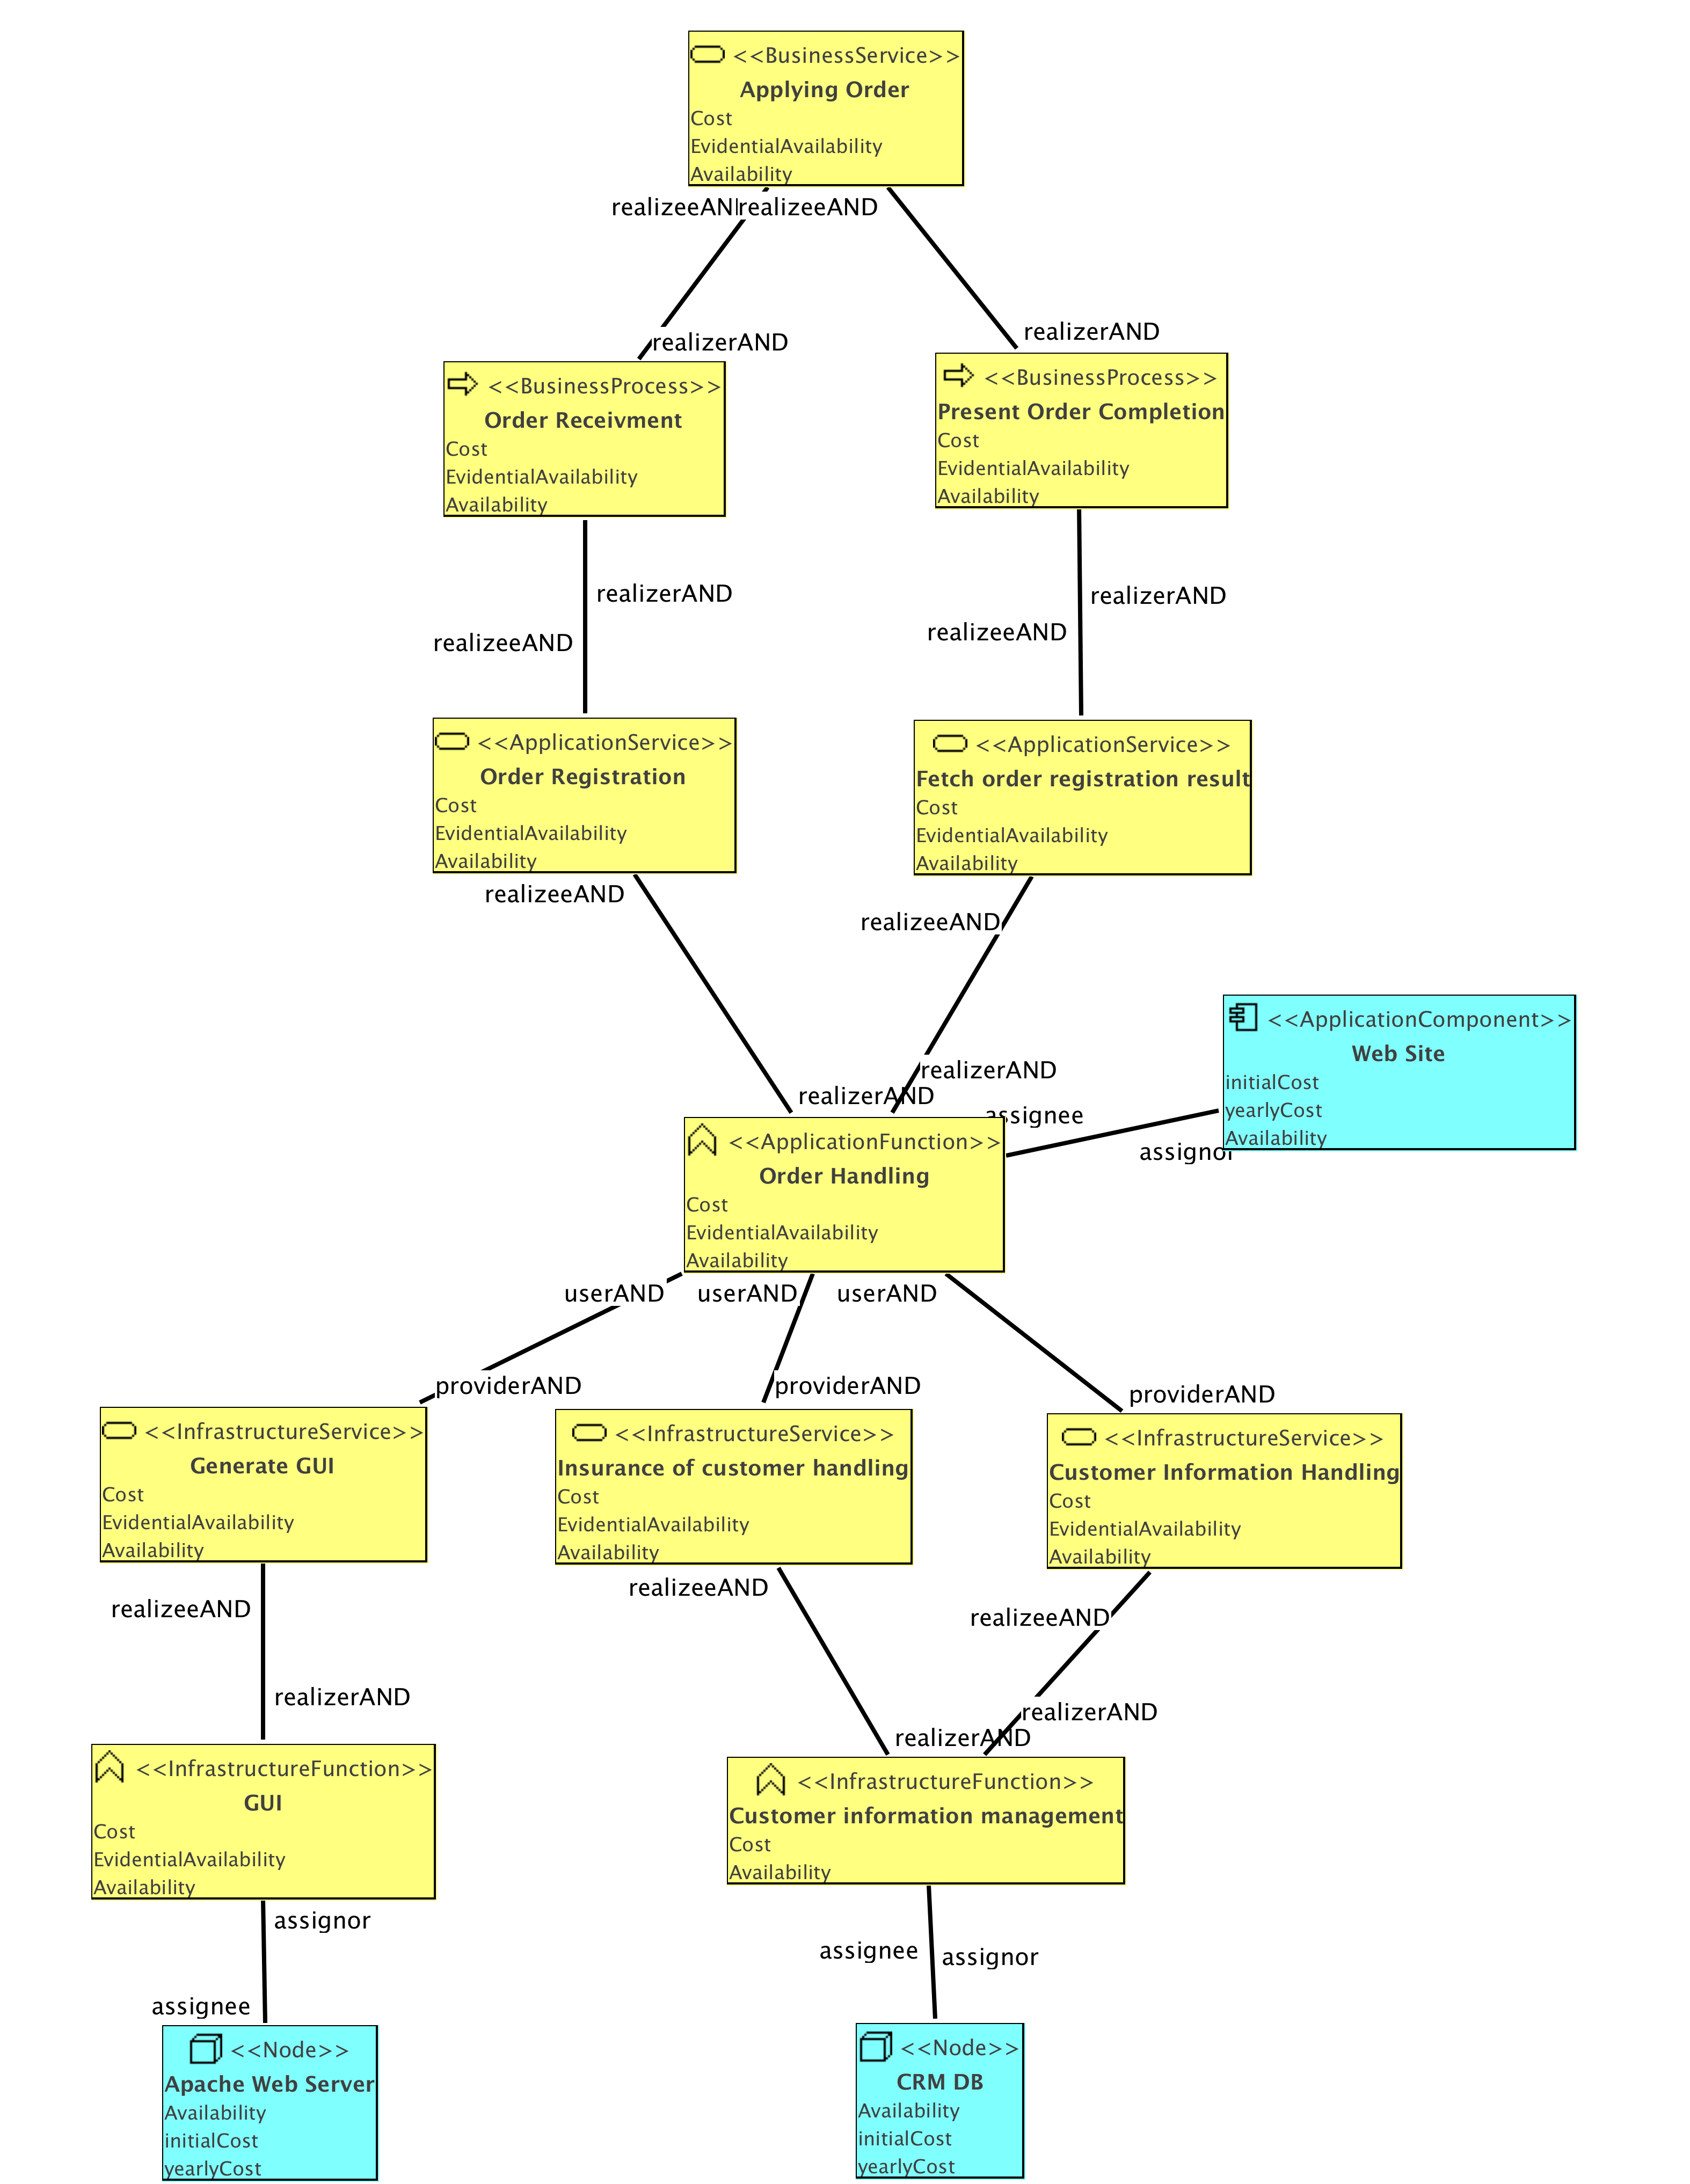
\includegraphics[scale = 0.07]{images/map_order_analysis_tobe.png}}
		\caption{\textsl{Cost} and \textsl{Service Availability} of the processes "Order Receivement" and "Present Order Completion"}
		\label{fig:map_order_cost_to_be}
	\end{figure}
\end{center}
The costs for the web site and the new implementations to it is an initial cost of 500 000 kr and has an yearly cost of 50 000 kr. The web server was an initial cost of 200 000 kr and a yearly cost of 20 000 kr, since the web server already existed in the company, no investment of the server had to be made. The CRM DB also already exists in the company and the initial cost for it was 700 000 kr and a yearly cost of 50 000 kr. This implies that the cost for the Order Registration Service and the Fetch Order Registration Result Service has a cost of 373 750 kr each. The availability of the Applying Order service is calculated to 0.90, from the availabilities of the systems. The values for the attributes Cost and availability for all objects in the view can be seen in \fref{tab:order_cost_to_be} and in \fref{tab:order_availability_to_be}.
\begin{table}[H]
	\centering
	\begin{tabular}{|c|c|p{2cm}|p{2.5cm}|p{2.5cm}|p{2.5cm}|}
		\cline{3-6}

		\multicolumn{2}{c}{} & \multicolumn{4}{|c|}{\textbf{Nodes}} \\ \cline{3-6}
		\multicolumn{2}{c|}{} & \multicolumn{2}{c|}{\textsl{CRM DB}} & \multicolumn{2}{c|}{\textsl{Apache Web Server}} \\
		\hline
		\multicolumn{2}{|c|}{\textbf{Initial Cost}} & \multicolumn{2}{c|}{700 000} & \multicolumn{2}{c|}{200 000} \\ \hline
		\multicolumn{2}{|c|}{\textbf{Yearly Cost}}  & \multicolumn{2}{c|}{50 000} & \multicolumn{2}{c|}{20 000} \\ \hline
		
		\multicolumn{6}{c}{} \\ \cline{3-6}
		\multicolumn{2}{c}{} & \multicolumn{4}{|c|}{\textbf{Application Component}} \\ \cline{3-6}
		\multicolumn{2}{c|}{} & \multicolumn{4}{c|}{\textsl{Web Site}} \\
		\hline
		\multicolumn{2}{|c|}{\textbf{Initial Cost}} & \multicolumn{4}{c|}{500 000}  \\ \hline
		\multicolumn{2}{|c|}{\textbf{Yearly Cost}}  & \multicolumn{4}{c|}{50 000}  \\ \hline

		\multicolumn{6}{c}{} \\ \cline{3-6}
		\multicolumn{2}{c}{} & \multicolumn{4}{|c|}{\textbf{Business Processes}} \\ \cline{3-6}
		\multicolumn{2}{c|}{} & \multicolumn{2}{c|}{\textsl{Order Receivement}} & \multicolumn{2}{c|}{\textsl{Present Order Completion}} \\
		\hline
		\multicolumn{2}{|c|}{\textbf{Cost}} & \multicolumn{2}{c|}{373 750} & \multicolumn{2}{c|}{373 750} \\ \hline
	\end{tabular}
\caption{Order process, \textsl{Cost} (To-Be)} 
\label{tab:order_to_be}
\end{table}
\emph{Note: We experienced some problem with EAAT calculating this, the cost when calculated was 0 but for the two supporting application services the cost was calculated. As the service is supported by two processes supported by each of these services, we just added the cost for the application services as the cost for the Applying Order.}
\begin{table}[H]
	\centering
	\begin{tabular}{|c|c|p{2cm}|p{2.5cm}|p{2.5cm}|p{2.5cm}|}
		\cline{3-6}

		\multicolumn{2}{c}{} & \multicolumn{4}{|c|}{\textbf{Nodes}} \\ \cline{3-6}
		\multicolumn{2}{c|}{} & \multicolumn{2}{c|}{\textsl{CRM DB}} & \multicolumn{2}{c|}{\textsl{Apache Web Server}} \\
		\hline
		\multicolumn{2}{|c|}{\textbf{Availability}}  & \multicolumn{2}{c|}{0.99} & \multicolumn{2}{c|}{0.99} \\ \hline
		
		\multicolumn{6}{c}{} \\ \cline{3-6}
		\multicolumn{2}{c}{} & \multicolumn{4}{|c|}{\textbf{Application Component}} \\ \cline{3-6}
		\multicolumn{2}{c|}{} & \multicolumn{4}{c|}{\textsl{Web Site}}  \\
		\hline
		\multicolumn{2}{|c|}{\textbf{Availability}} & \multicolumn{4}{c|}{0.99}  \\ \hline
		
		\multicolumn{6}{c}{} \\ \cline{3-6}
		\multicolumn{2}{c}{} & \multicolumn{4}{|c|}{\textbf{Business Processes}} \\ \cline{3-6}
		\multicolumn{2}{c|}{} & \multicolumn{2}{c|}{\textsl{Order Registration}} & \multicolumn{2}{c|}{\textsl{Present Order Completion}} \\
		\hline
		\multicolumn{2}{|c|}{\textbf{Availability}} & \multicolumn{2}{c|}{0.96} & \multicolumn{2}{c|}{0.96} \\ \hline

		\multicolumn{6}{c}{} \\ \cline{3-6}
		\multicolumn{2}{c}{} & \multicolumn{4}{|c|}{\textbf{Business Services}} \\ \cline{3-6}
		\multicolumn{2}{c|}{} &  \multicolumn{4}{c|}{\textsl{Applying Order}}  \\
		\hline
		\multicolumn{2}{|c|}{\textbf{Availability}}  & \multicolumn{4}{c|}{0.92}\\ \hline
	\end{tabular}
\caption{Order process, \textsl{Service Availability} (To-Be)} 
\label{tab:order_as_is}
\end{table}

\subsubsection{Claim Registration - Data Accuracy}
The changes to the claim registration process impacted the structure of the data written to the systems. The Claim registration process is now automated and the written description by the user on the website is read and written by the system in digital formats. The new write and read flow of the representation and data sets can be viewed in \fref{fig:map_claim_data_to_be}. 
\label{sec:claim_analysis_to_be}
	\begin{center}
		\begin{figure}[H]
			\centering
			\setlength\fboxsep{7pt}
			\setlength\fboxrule{0.5pt}
			\fbox{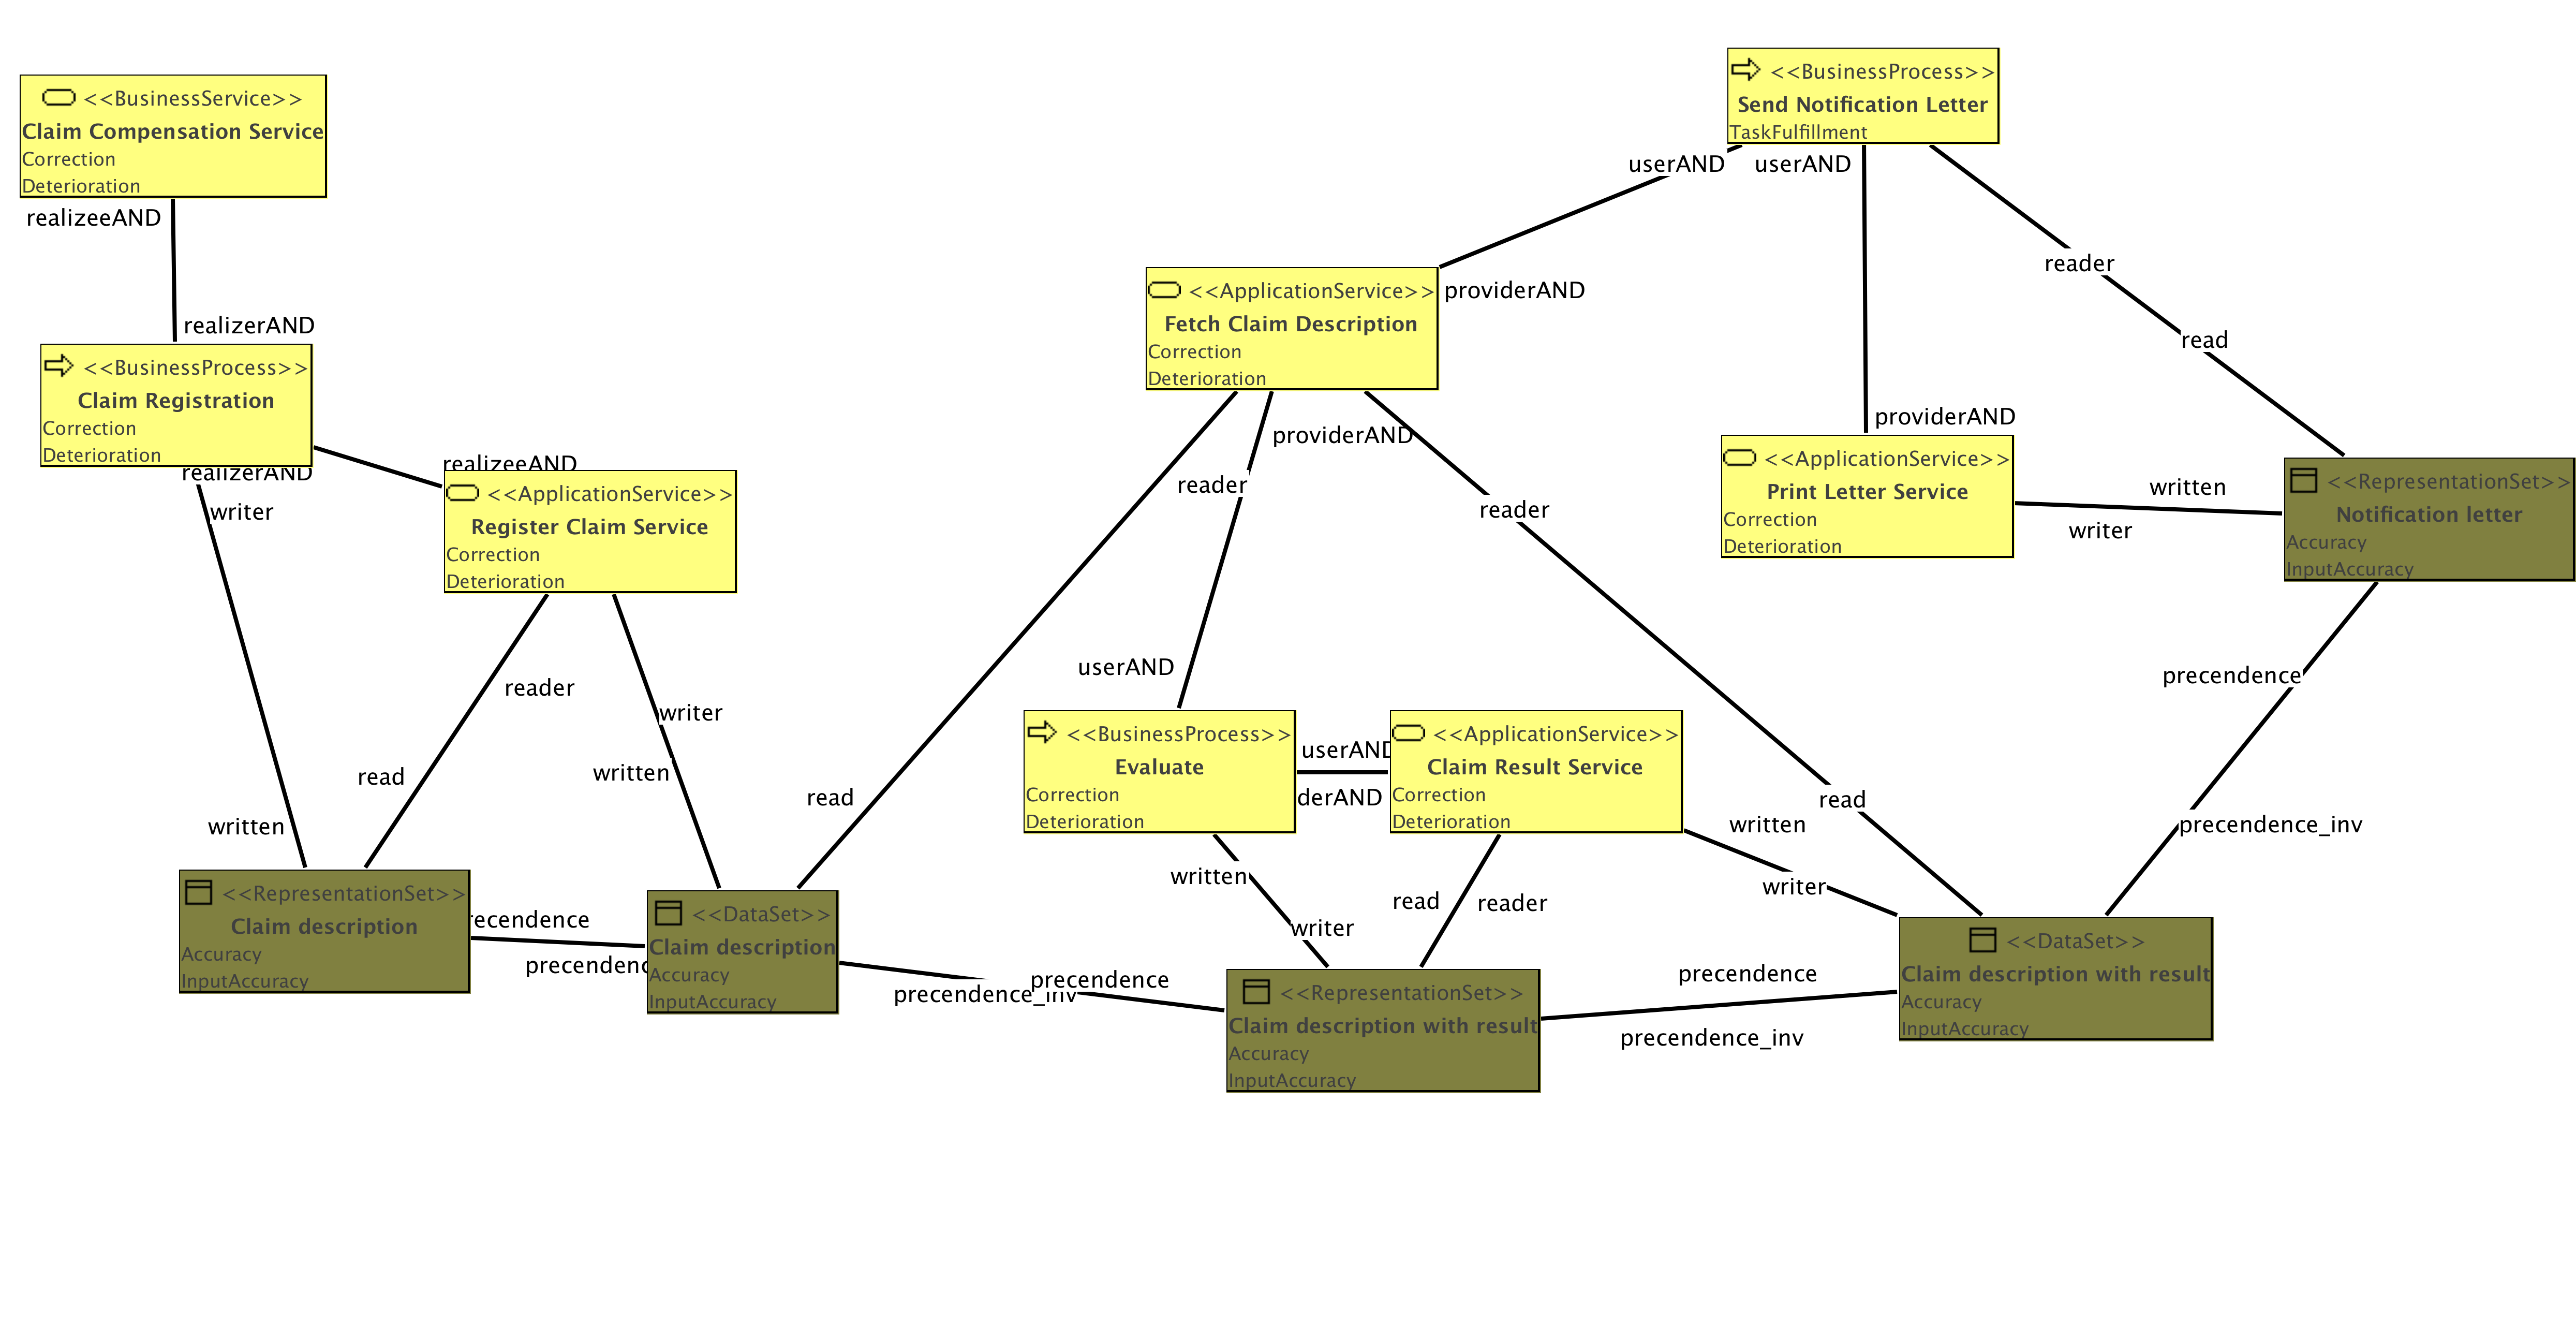
\includegraphics[scale = 0.07]{images/map_claim_analysis_tobe.png}}
			\caption{\textsl{Data Accuracy} for the Claim Process}
			\label{fig:map_claim_data_to_be}
		\end{figure}
	\end{center}
	The process "Claim Registration" has now a decreased value of deterioration to 0.01 since the process is automated on the website. This impact the accuracy of the stored claim description (data set) to the better, which now is 0.97. The accuracy of the Notification letter in the end of the process is calculated to 0.92. \Fref{tab:claim_to_be} shows the values of the involved objects and the resulting accuracy of the representation sets and the data sets.
\begin{center}
\begin{table}[H]
\begin{tabular}{|c|c|p{2cm}|p{2.5cm}|p{2.5cm}|p{2.5cm}|}

%\textbf{Attribute}& \textbf{State} & \textsl{Claim Application} & \textsl{Claim Description} & \textsl{Claim Description with result} & \textsl{Notification letter} \\

\cline{3-6}
\multicolumn{2}{c}{} & \multicolumn{4}{|c|}{\textbf{Nodes}} \\ \cline{3-6}
\multicolumn{2}{c|}{} & \textsl{Claim Application} & \textsl{Claim Description} & \textsl{Claim Description with Result} & \textsl{Notification Letter}\\
\hline
\multirow{2}{*}{Input Accuracy} & As-Is & \multicolumn{1}{c|}{0.99} & \multicolumn{1}{c|}{0.98} & \multicolumn{1}{c|}{0.99} & \multicolumn{1}{c|}{0.99}\\ \cline{2-6}
								& To-Be & \multicolumn{1}{c|}{0.99} & \multicolumn{1}{c|}{0.98} & \multicolumn{1}{c|}{0.99} & \multicolumn{1}{c|}{0.99}\\ \hline

\multirow{2}{*}{Accuracy} 		& As-Is & \multicolumn{1}{c|}{0.99} & \multicolumn{1}{c|}{0.84} & \multicolumn{1}{c|}{0.80} & \multicolumn{1}{c|}{0.79}\\ \cline{2-6}
								& To-Be & \multicolumn{1}{c|}{0.99} & \multicolumn{1}{c|}{0.98} & \multicolumn{1}{c|}{0.93} & \multicolumn{1}{c|}{0.92}\\ \hline

\multicolumn{6}{c}{} \\ \cline{3-6}
\multicolumn{2}{c}{} & \multicolumn{4}{|c|}{\textbf{Business process}} \\ \cline{3-6}
\multicolumn{2}{c|}{} & \multicolumn{4}{|c|}{\textsl{Claim Registration}} \\ \hline
\multirow{2}{*}{Deterioration} & As-Is & \multicolumn{4}{|c|}{0.15}\\ \cline{2-6}
							   & To-Be & \multicolumn{4}{|c|}{0.01}\\ \hline
\end{tabular}
\caption{Claim process, \textsl{Data accuracy} To-Be}
\label{tab:claim_to_be}
\end{table}
\end{center}
%
\subsubsection{Support - Service Availability}
The aggregation of the phone support service and the mail support service into one support service to increase the availability can be viewed in \fref{fig:map_support_combined_availability_to_be}. The Helpdesk System now enables the support processes and the existing phone dispatcher system and the mailserver are used by the new system. The employees executing today's processes are aggregated to a new role as Helpdesk employee.
\label{sec:support_analysis_to_be}
\begin{center}
	\begin{figure}[H]
		\centering
		\setlength\fboxsep{7pt}
		\setlength\fboxrule{0.5pt}
		\fbox{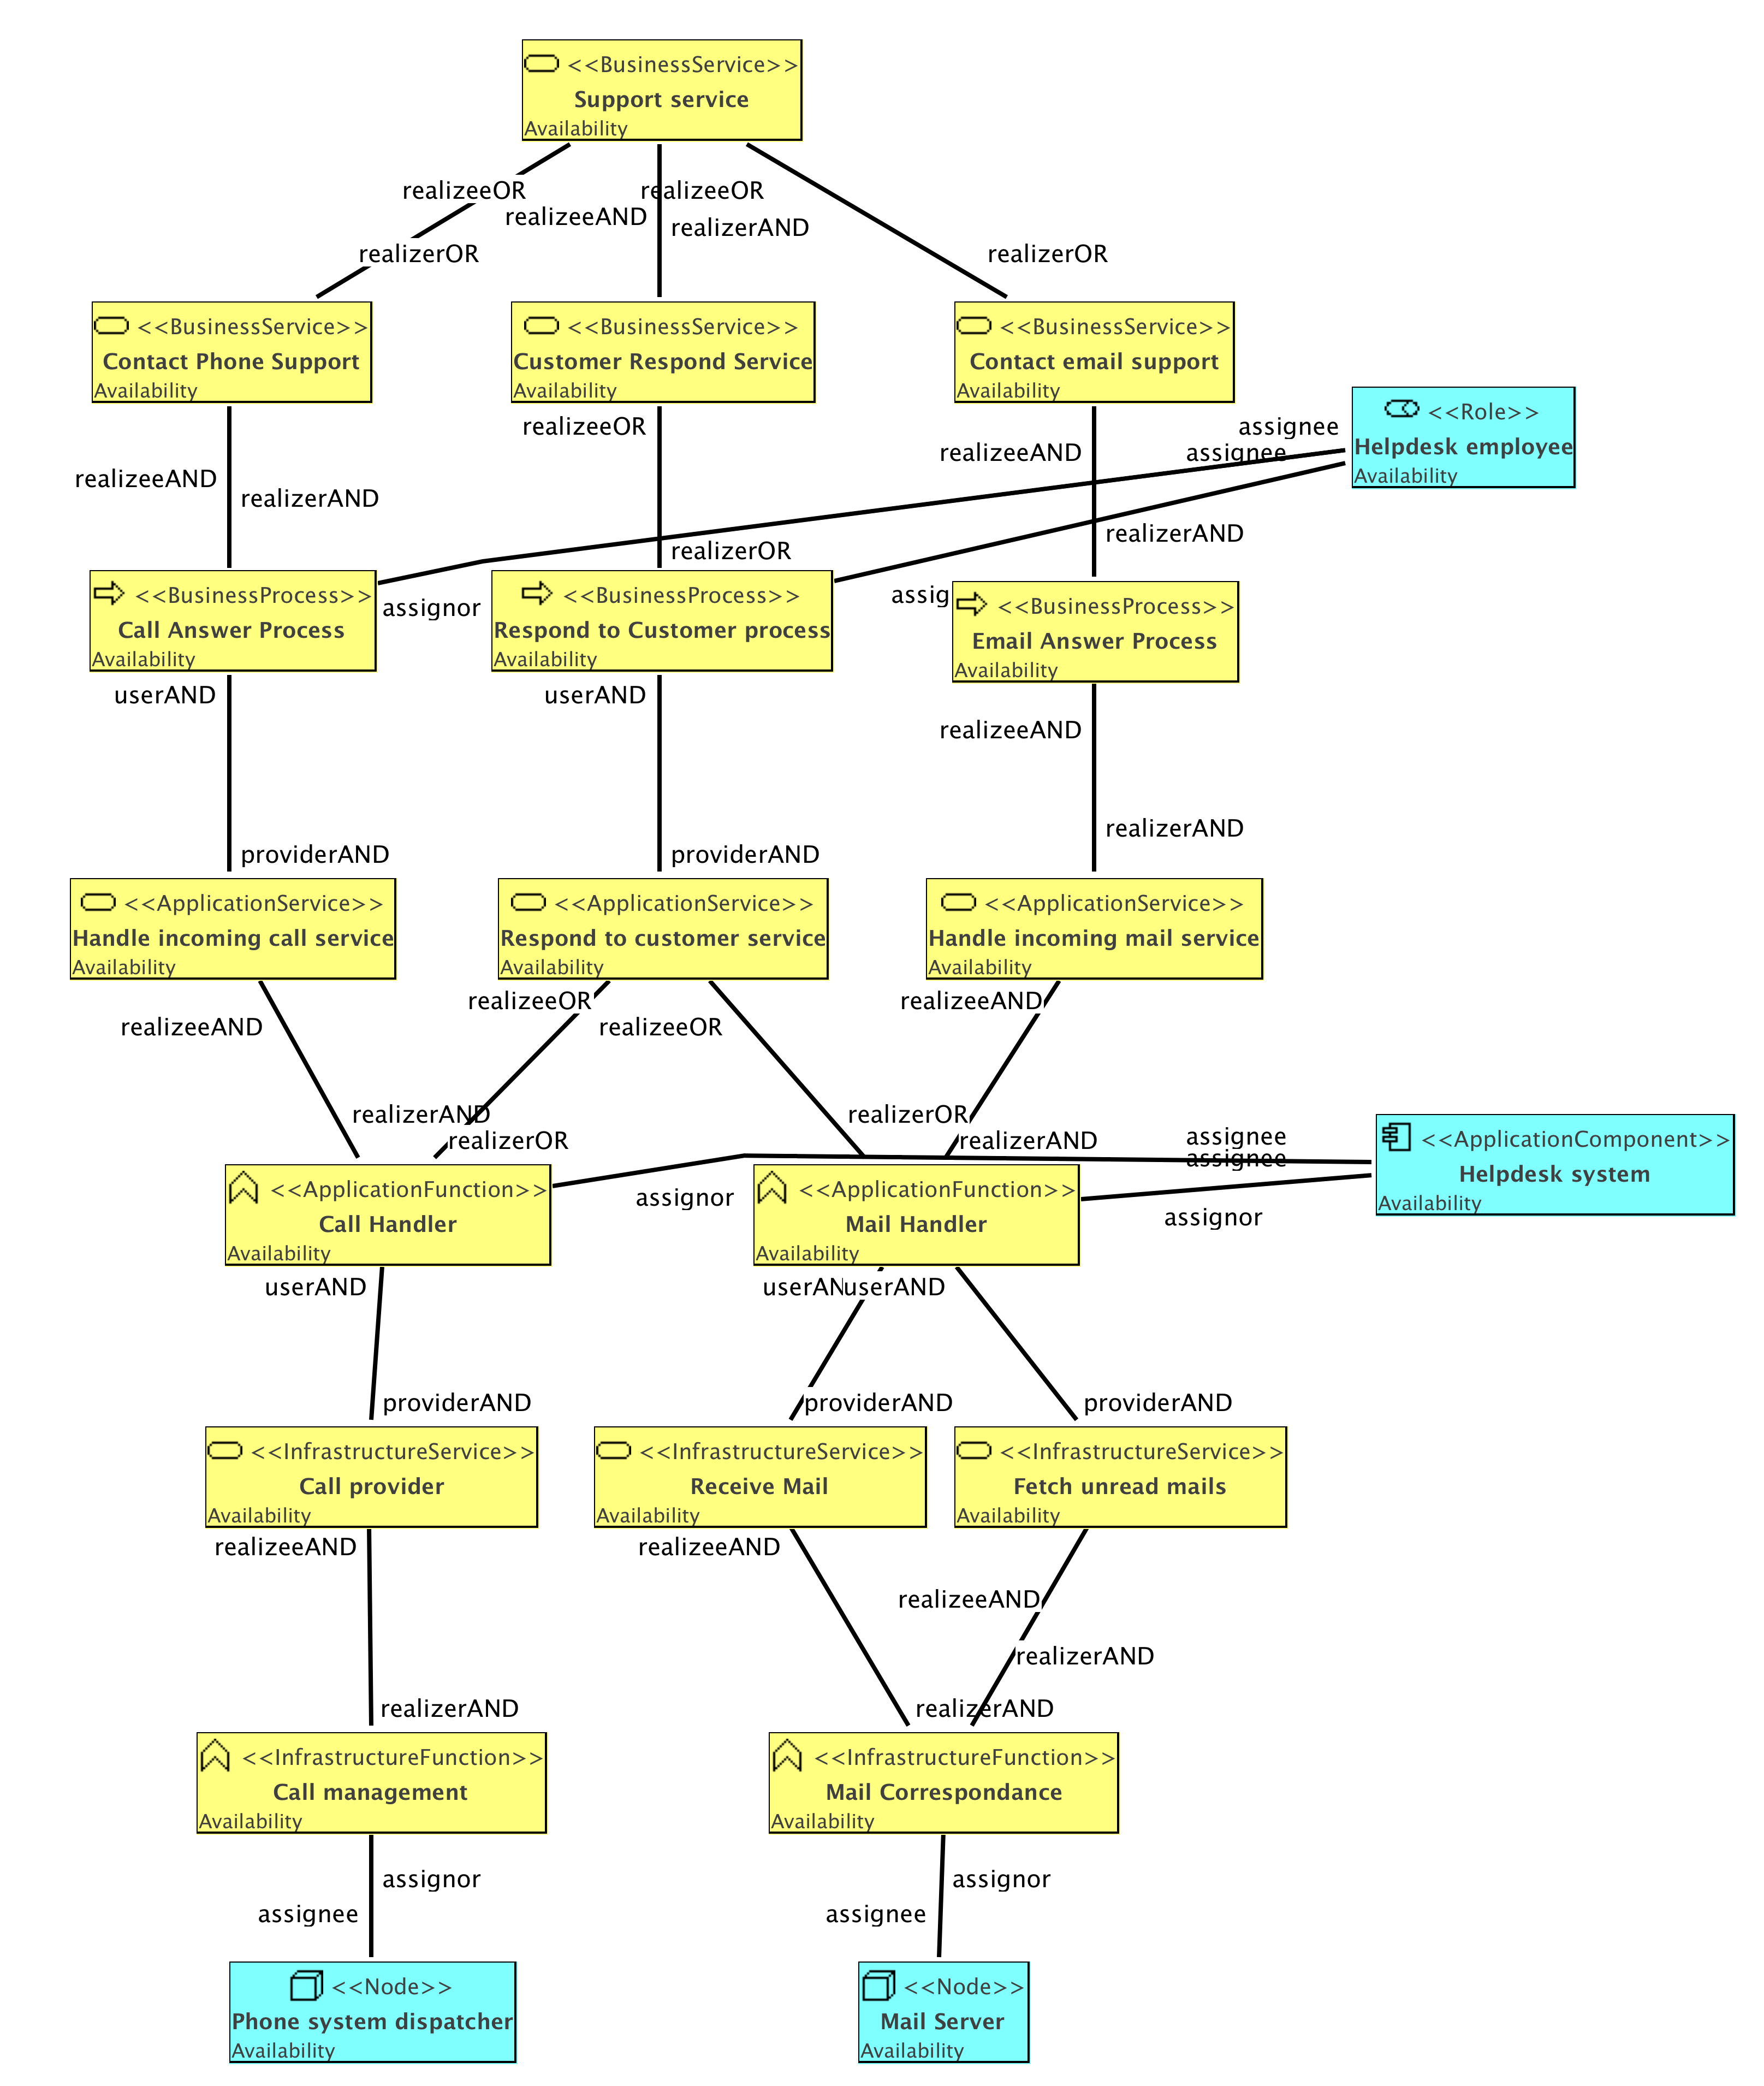
\includegraphics[scale = 0.07]{images/map_analysis_support_tobe.png}}
		\caption{\textsl{Service Availability} of the new support process}
		\label{fig:map_support_combined_availability_to_be}
	\end{figure}
\end{center}
The Phone system dispatcher and the Mail Server are the same as the one now operating. The new Helpdesk system would have an availability of 0.99 and the more flexible Helpdesk employees an availability of 0.97. The Contact Phone Support service then gets an availability of 0.93, the Contact Email Support service an availability of 0.95 and the Customer Respond Service an availability of 0.99. \Fref{tab:support_to_be} views all the availabilities of the systems and the processes.
\begin{table}[H]
	\centering
	\begin{tabular}{|c|c|p{2.5cm}|p{2.5cm}|p{2.5cm}|p{2.5cm}|}

		%\multicolumn{2}{c}{} & \multicolumn{1}{p{2.5cm}}{} & \multicolumn{2}{p{5cm}}{} & \multicolumn{1}{p{2.5cm}}{} \\ %ALLIGNER!
		\cline{3-6}

		\multicolumn{2}{c}{} & \multicolumn{4}{|c|}{\textbf{Nodes}} \\ \cline{3-6}
		\multicolumn{2}{c|}{} & \multicolumn{1}{|c|}{\textsl{Phone System Dispatcher}} & \multicolumn{2}{|c|}{\textsl{Mail Server}} &\multicolumn{1}{|c|}{\textsl{Help Desk DB}} \\ \hline
		\multicolumn{2}{|c|}{\textbf{Availability}} & \multicolumn{1}{|c|}{0.97} & \multicolumn{2}{|c|}{0.97} & \multicolumn{1}{|c|}{0.99} \\  \hline

		\multicolumn{6}{c}{} \\ \cline{3-6}							
		\multicolumn{2}{c}{} & \multicolumn{4}{|c|}{\textbf{Application Components}} \\ \cline{3-6}
		\multicolumn{2}{c|}{} & \multicolumn{4}{c|}{\textsl{Help Desk System}} \\
		\hline
		\multicolumn{2}{|c|}{\textbf{Availability}} & \multicolumn{4}{c|}{0.99} \\ \hline

	   \multicolumn{6}{c}{} \\ \cline{3-6}
		\multicolumn{2}{c}{} & \multicolumn{4}{|c|}{\textbf{Role}} \\ \cline{3-6}
		\multicolumn{2}{c|}{} & \multicolumn{4}{|c|}{\textsl{Help Desk Supporter}}\\ \hline
		\multicolumn{2}{|c|}{\textbf{Availability}}& \multicolumn{4}{|c|}{0.97} \\  \hline
		
		\multicolumn{6}{c}{} \\ \cline{3-6}
		\multicolumn{2}{c}{} & \multicolumn{4}{|c|}{\textbf{Business Services}} \\ \cline{3-6}
		\multicolumn{2}{c|}{} & \multicolumn{1}{|c|}{\textsl{Contact Phone Support}} & \multicolumn{2}{|c|}{\textsl{Contact Email Support}} & \multicolumn{1}{|p{2cm}|}{\textsl{Respond to Customer}}\\ \hline
		\multicolumn{2}{|c|}{\textbf{Availability}}& \multicolumn{1}{|c|}{0.93} & \multicolumn{2}{|c|}{0.94} & \multicolumn{1}{|c|}{0.97}\\ \hline
	\end{tabular}
\caption{Support process, \textsl{Service Availability} (To-Be)} 
\label{tab:support_to_be}
\end{table}
%







